\documentclass[11pt,a4paper]{article}

\usepackage[utf8]{inputenc}
\usepackage[T1]{fontenc}
\usepackage{lmodern}
\usepackage[margin=1in]{geometry}
\usepackage{amsmath,amssymb,amsfonts}
\usepackage{booktabs}
\usepackage{array}
\usepackage{graphicx}
\usepackage{hyperref}
\usepackage{authblk}
\usepackage{caption}
\usepackage{float}
\usepackage{tabularx}
\usepackage{ragged2e}
\usepackage{url}
\usepackage{tikz}
\usetikzlibrary{arrows.meta,positioning}
\usepackage{makecell}
\usepackage{microtype}

\hypersetup{
    colorlinks=true,
    linkcolor=blue,
    citecolor=blue,
    urlcolor=blue
}

% Title and Author Block
\title{\textbf{An IoT-Based Infrastructure Model for Reducing Urban Light Pollution: Empirical Assessment and System Design in Dhaka}}

\author[1]{Md Reyad Hasan\thanks{Corresponding author: \texttt{reyadh418@gmail.com}}}
\author[2]{Ishrat Jahan Riya\thanks{Email: \texttt{ishratjahanriya123@gmail.com}}}

\affil[1]{Government Science College, Dhaka, Bangladesh}
\affil[2]{Mavenwood International School, Dhaka, Bangladesh}

\date{August 23, 2026}

\begin{document}

\maketitle

\begin{abstract}
\noindent Unregulated artificial light at night (ALAN) in rapidly expanding megacities drives severe atmospheric skyglow, circadian disruption, ecological degradation, and municipal energy waste. Despite its severity across South Asia, ground-level photometric data in developing urban centers remains scarce, and municipal streetlighting continues to rely on static, all-night full-beam operation. In this study, we first establish an empirical baseline of urban light pollution in Dhaka, Bangladesh, by conducting 220 in-situ lux measurements across 13 distinct urban sectors, paired with 12 controlled benchtop luminaire experiments. Field audits reveal an overall mean illuminance of 802.5~lx and expose extreme spatial disparities: while residential, educational, and office zones average between 61.5~lx and 79.5~lx, unshielded commercial facades in fashion retail (mean: 1,401.3~lx; peak: 4,925.0~lx), electronics markets (mean: 1,458.4~lx; peak: 3,200.0~lx), and shopping complexes (peak: 4,303.0~lx) exceed international roadway safety thresholds by up to \(164\times\). Concurrently, municipal roadways fluctuate erratically between hazardous dark zones (5.0~lx) and over-illuminated junctions (500.0~lx; mean: 74.0~lx). To eliminate continuous nocturnal over-illumination without compromising public safety, we design an autonomous, decentralized Internet of Things (IoT) streetlight infrastructure that generates a predictive ``rolling luminescence bubble.'' Each lamppost is partitioned into four vertical hardware zones managed by an ESP32-S3 Sense microcontroller utilizing SIMD vector acceleration to fuse seven sensing modalities: an OV2640 edge camera running quantized TinyML vision models (YOLOv8-nano/MobileNet), an HB100 microwave Doppler radar for long-range approach velocity tracking, a sidewalk-directed passive infrared (PIR) array, a sky-facing BH1750 ambient light sensor, a BME280 atmospheric weather module, a DS3231 temperature-compensated real-time clock (RTC), and an INA219 power telemetry monitor. By bypassing heavy TCP/IP stacks in favor of connectionless OSI Layer-2 ESP-NOW broadcasts (\(<10\)~ms latency), nodes project an illuminated safety envelope 30--40~m ahead of approaching vehicles at 100\% pulse-width modulation (PWM) output, maintain localized 40\%--50\% envelopes for pedestrians, and execute a smooth 3--5~s linear decay back to a 10\% eco-baseline after departure. System reliability is guaranteed through a deterministic six-tier priority conflict-resolution matrix, automated post-midnight 50\% skyglow curfews, weather-adaptive baseline scaling, and a 100\% full-beam fail-safe fallback during hardware anomalies.
\end{abstract}

\vspace{0.5em}
\noindent\textbf{Keywords:} Light Pollution, Smart Streetlighting, Edge AI, Sensor Fusion, ESP-NOW Mesh, ESP32-S3, Urban Sustainability, Dhaka.

\section{Introduction}

\subsection{Background and Urban Context}
Artificial light at night (ALAN) is foundational to modern urban infrastructure, supporting road safety, pedestrian mobility, and nocturnal commerce. However, the rapid, uncalibrated transition to high-intensity solid-state light-emitting diodes (LEDs)---frequently installed without optical cutoff shielding, spectral filtering, or demand-responsive dimming---has transformed urban lighting into a pervasive environmental pollutant \cite{falchi2016new,kyba2017artificially,sanchez2021first,darksky_ies2020}. Unmitigated ALAN manifests through three primary mechanisms: upward-radiated \textit{skyglow} scattered by atmospheric aerosols and moisture, horizontal \textit{light trespass} penetrating residential windows, and direct ocular \textit{glare} that degrades night vision contrast. Beyond wasting substantial municipal electricity, chronic exposure to high-intensity nocturnal lighting suppresses human melatonin synthesis, disrupts circadian regulation \cite{cho2015effects}, and alters the navigation, foraging, and reproductive cycles of urban fauna \cite{gaston2013ecological}.

In densely populated, fast-growing South Asian metropolises such as Dhaka, Bangladesh, nocturnal illumination operates without photometric standardization or adaptive control. Municipal thoroughfares, flyovers, hospital perimeters, and commercial corridors rely on static switching regimes that lock luminaires at 100\% output from dusk until dawn. Consequently, empty streets at 3:00~AM receive the exact same luminous flux as congested intersections during peak evening rush hours.

\subsection{Empirical Motivation: The Dhaka Photometric Audit}
To ground our infrastructure design in real-world urban conditions, we conducted a systematic field survey across major neighborhoods in Dhaka (including Shyamoli, Mirpur, Mohammadpur, Kallyanpur, Kawran Bazar, Farmgate, Shahbagh, Shere Bangla Nagar, and Jatrabari), capturing \(N = 220\) site measurements across 13 functional urban sectors alongside 12 controlled benchtop prototype trials. 

\begin{table}[tbp]
\centering
\caption{Summary of Empirical Illuminance Measurements Across 13 Urban Sectors in Dhaka (\(N = 220\)). \normalfont{\footnotesize{Note: Mean, Median, and Std.\ Dev.\ are computed across site-level spatial averages, whereas Min and Max reflect the extreme directional bounds (\textit{Lower} and \textit{Higher Range}) recorded within each sector.}}}
\label{tab:dhaka_summary}
\small
\setlength{\tabcolsep}{5pt}
\begin{tabular}{l c r r r r r}
\toprule
\textbf{Urban Sector} & \textbf{Sites (\(n\))} & \textbf{Mean (lx)} & \textbf{Median (lx)} & \textbf{Std.\ Dev.} & \textbf{Min (lx)} & \textbf{Max (lx)} \\
\midrule
Fashion & 62 & 1401.3 & 1400.0 & 781.4 & 16.6 & 4925.0 \\
Variety Shop & 32 & 800.0 & 650.0 & 590.0 & 5.0 & 3841.0 \\
Food and Restaurants & 26 & 534.4 & 417.5 & 596.1 & 80.0 & 4375.0 \\
Roads & 21 & 74.0 & 50.0 & 81.4 & 5.0 & 500.0 \\
Mobile and Accessories & 20 & 1458.4 & 1473.5 & 566.5 & 250.0 & 3200.0 \\
Hospital & 14 & 355.1 & 175.5 & 369.1 & 30.0 & 1300.0 \\
Super Shop \& Convention Hall & 13 & 755.9 & 339.7 & 670.7 & 42.0 & 4303.0 \\
Buildings \& Residence & 11 & 79.5 & 65.0 & 58.1 & 16.0 & 290.0 \\
School, Coaching \& Learning & 9 & 65.1 & 48.0 & 58.9 & 7.0 & 215.0 \\
Cars and Transportation & 6 & 652.7 & 500.0 & 584.5 & 2.3 & 1511.0 \\
Cinemas \& Entertainments & 3 & 249.6 & 351.0 & 183.5 & 25.8 & 843.0 \\
Office & 2 & 61.5 & 61.5 & 26.2 & 28.0 & 128.0 \\
Visitable Places \& Heritages & 1 & 88.0 & 88.0 & 0.0 & 65.0 & 119.0 \\
\midrule
\textbf{Total / Overall} & \textbf{220} & \textbf{802.5} & --- & --- & \textbf{2.3} & \textbf{4925.0} \\
\bottomrule
\end{tabular}
\end{table}

As detailed in Table~\ref{tab:dhaka_summary}, our empirical audit identifies three critical structural deficiencies in Dhaka's current lighting landscape:
\begin{enumerate}
    \item \textbf{Extreme Commercial Light Trespass:} Across all 220 surveyed locations, mean illuminance reached 802.5~lx---more than \(26\times\) the maximum 30.0~lx level recommended by Illuminating Engineering Society (IES RP-8) guidelines \cite{ies_rp8} for urban collector roadways. This saturation is driven by unshielded commercial storefronts that spill intense horizontal flux directly onto public sidewalks and adjacent residential buildings. Fashion retail outlets averaged 1,401.3~lx with peaks of 4,925.0~lx (\(164.2\times\) the 30.0~lx roadway benchmark), mobile and accessories markets averaged 1,458.4~lx (peaking at 3,200.0~lx), and shopping complexes reached 4,303.0~lx.
    \item \textbf{Erratic and Uncalibrated Roadway Illumination:} Across 21 surveyed roadway and transit segments, average illuminance was 74.0~lx (median: 50.0~lx), but spatial uniformity was severely compromised. Readings fluctuated from hazardous, unlit pockets of 5.0~lx at transit stops to glaring 500.0~lx concentrations (\(16.7\times\) standard guidelines) along main arterial corridors, with zero dynamic dimming during low-traffic nocturnal windows.
    \item \textbf{Fixture Geometry and Spectral Spill:} Our 12 controlled benchtop experiments demonstrated that luminaire mounting geometry and spectral selection directly govern stray light propagation. Elevating the luminaire and shifting orientation from a \(90^\circ\) vertical emission (632.4~lx average) to a taller horizontal-cutoff profile (261.7~lx average) reduced concentrated ground hotspot intensity by 58.6\%. Furthermore, short-wavelength blue emitters generated severe peak glare (865.5~lx) compared to warm yellow/orange LEDs (455.5~lx), while specialized tinted window glazing reduced indoor light trespass by 46.7\% (from 122.3~lx down to 65.2~lx) relative to standard transparent glass.
\end{enumerate}

\subsection{Bottlenecks in Conventional Smart Streetlighting}
Although adaptive streetlighting has been widely explored in academic literature \cite{castro2013smart,lau2015traffic}, translating theoretical designs into reliable urban infrastructure faces three technical bottlenecks:
\begin{itemize}
    \item \textbf{Single-Modal Sensing Failures:} Architectures dependent solely on Passive Infrared (PIR) or ultrasonic transducers are constrained by short detection horizons (\(<10\)~m) and frequent false activations triggered by wind-blown foliage, stray animals, or convective heat plumes. Conversely, camera-only architectures degrade under heavy glare, rain, or fog and impose prohibitive computational loads on low-cost microcontrollers.
    \item \textbf{Protocol Latency vs. Stopping Sight Distance:} A vehicle traveling at 60~km/h (16.7~m/s) requires an illuminated look-ahead horizon of 30--40~m to guarantee safe stopping sight distance. Smart lighting networks built on centralized cloud brokers, cellular links, or multi-hop TCP/IP Wi-Fi meshes incur 100--300~ms latencies, causing downstream luminaires to ramp up \textit{after} a fast-moving vehicle has already entered the dark sector.
    \item \textbf{Absence of Multi-Sensor Conflict Arbitration:} Basic motion-activated streetlights lack formal decision hierarchies to resolve contradictory or simultaneous events---such as a high-speed vehicle and a stationary pedestrian sharing a sector, sudden sensor dropout mid-sequence, atmospheric visibility drops during storms, or post-midnight skyglow curfews.
\end{itemize}

\subsection{Proposed Infrastructure Model and Contributions}
To resolve these challenges, we present an IoT-based smart streetlight infrastructure that replaces static all-night lighting with an adaptive, peer-to-peer \textbf{rolling luminescence bubble}. Luminaires idle at a 10\% eco-baseline and dynamically modulate their pulse-width modulation (PWM) duty cycle in real time according to target classification, approach velocity, local meteorology, and chronological curfew gates. The primary contributions of this work are fourfold:
\begin{enumerate}
    \item \textbf{Comprehensive Urban Illuminance Dataset:} We provide an empirical 220-site multi-sector photometric dataset of Dhaka alongside 12 controlled fixture experiments, quantifying the severity of commercial light trespass and roadway over-illumination in a developing megacity.
    \item \textbf{Four-Zone Edge AI Sensor-Fusion Architecture:} We engineer a vertically stratified lamppost node around the dual-core ESP32-S3 Sense microcontroller (leveraging hardware SIMD vector instructions) \cite{espressif_esp32s3}, integrating an OV2640 camera running quantized TinyML vision models (YOLOv8-nano \cite{redmon_yolo} / MobileNet \cite{howard2017mobilenets}), an HB100 microwave Doppler radar, a sidewalk-level PIR array, a sky-facing BH1750 ambient light sensor, a BME280 atmospheric sensor, a DS3231 real-time clock, and an INA219 inline power monitor.
    \item \textbf{Sub-10~ms Predictive Look-Ahead via ESP-NOW:} By operating directly on the OSI Data-Link Layer via connectionless ESP-NOW action frames \cite{espressif_espnow}, detecting nodes broadcast target velocity and heading to downstream neighbors in \(<10\)~ms, illuminating roadway segments 30--40~m ahead of approaching vehicles and executing a 3--5~s linear decay upon departure to eliminate rearview strobe effects.
    \item \textbf{Deterministic Priority Arbitration and Fail-Safe State Machine:} We formulate a six-rank sensor conflict-resolution hierarchy and an edge-case fault-tolerance table that arbitrate simultaneous vehicle-pedestrian encounters, enforce post-midnight 50\% PWM skyglow curfews, elevate safety floors to 60\% during low-visibility storms, reject non-human/vehicle false triggers via TinyML spectral filtering, and enforce a 100\% full-beam fail-safe fallback upon sensor dropout.
\end{enumerate}

\section{Empirical Field Assessment and Benchtop Photometric Analysis}

\subsection{Field Audit Protocol and Spatial Scope}
To establish a quantitative baseline of urban light pollution prior to designing our adaptive IoT control architecture, we conducted a systematic nocturnal photometric audit across \(N = 220\) measurement locations spanning 13 functional urban sectors in Dhaka, Bangladesh (primarily encompassing Shyamoli, Mirpur-1, Mirpur-2, Mohammadpur, Kallyanpur, Kawran Bazar, Farmgate, Shahbagh, Shere Bangla Nagar, Kakrail, Saydabad, and Jatrabari), alongside suburban and rural control baselines in Gazipur and Cumilla. 

At each site, illuminance (expressed in lux, \(\text{lx} = \text{lm/m}^2\)) was measured using a calibrated digital lux meter across multiple spatial orientations to capture minimum (\textit{Lower Range}), maximum (\textit{Higher Range}), and spatial mean (\textit{Average}) illuminance values. For each observation, the exact site identity, urban zone, sensor placement geometry (e.g., middle of roadway, sidewalk/footpath level, building entrance, or indoor/outdoor boundary), and dominant visual spectral emission color were recorded. To complement the urban field campaign, we also executed 12 controlled benchtop photometric trials to isolate the effects of luminaire tilt angle, mounting height, LED spectral wavelength, optical shielding geometry, and window glazing transmittance.

\subsection{Cross-Sectoral Analysis of Urban Light Pollution}

\subsubsection{Commercial Hyper-Illumination and Lateral Light Trespass}
The field dataset reveals that commercial retail zones are the dominant drivers of nocturnal over-illumination and lateral light trespass in Dhaka. While international outdoor lighting standards (such as IES RP-8 \cite{ies_rp8}, CIE 115 \cite{cie115}, and CIE 150 \cite{cie150}) recommend between 10.0~lx and 50.0~lx for commercial pedestrian corridors and urban roadways, surveyed retail storefronts routinely operate two orders of magnitude above these thresholds:
\begin{itemize}
    \item \textbf{Fashion and Apparel Outlets (\(n = 62\)):} This sector exhibited an average mean illuminance of 1,401.3~lx (\(\text{median} = 1,400.0\text{ lx}\), \(\sigma = 781.4\text{ lx}\)). Extreme localized peaks were recorded at major retail storefronts, including \textit{Infinity} (4,925.0~lx peak; 2,000.0~lx mean), \textit{Rongpolli} (4,806.0~lx peak; 2,108.0~lx mean), \textit{Easy Fashions} (4,600.0~lx peak; 2,300.0~lx mean), \textit{Cats Eye} (4,493.0~lx peak; 2,900.0~lx mean), and \textit{Illiyen} at Bashundhara City (4,000.0~lx peak).
    \item \textbf{Mobile and Electronics Showrooms (\(n = 20\)):} Electronics corridors recorded the highest sector-wide mean average at 1,458.4~lx (\(\text{median} = 1,473.5\text{ lx}\), \(\sigma = 566.5\text{ lx}\)), led by \textit{Tecno} in Mirpur-1 (3,200.0~lx peak; 2,960.0~lx mean) and \textit{Xiaomi} outlets (up to 2,500.0~lx peak; 1,710.0~lx mean).
    \item \textbf{Super Shops, Variety Stores, and Dining (\(n = 71\) combined):} Super shops and shopping malls (\(n = 13\)) averaged 755.9~lx, with severe outward flux at \textit{Prince Bazar} (4,303.0~lx peak; 1,693.0~lx mean) and the main entrance of \textit{Bashundhara Shopping Complex} in Kawran Bazar (2,500.0~lx peak; 1,900.0~lx mean). Variety shops (\(n = 32\)) averaged 800.0~lx (peaking at 3,841.0~lx), while food and restaurant establishments (\(n = 26\)) averaged 534.4~lx, peaking at 4,375.0~lx (3,200.0~lx mean) at an unshielded juice storefront in Town Hall, Mohammadpur.
\end{itemize}

Because these commercial arrays utilize unshielded, high-wattage LED floodlights mounted perpendicular to storefronts, their luminous flux spills directly across sidewalks and into adjacent roadways and residential upper floors.

\subsubsection{Roadway Non-Uniformity and Vehicular Glare Dynamics}
Across the \(n = 21\) surveyed roadway and transit locations, mean illuminance was 74.0~lx (\(\text{median} = 50.0\text{ lx}\), \(\sigma = 81.4\text{ lx}\)), spanning a \(100\times\) dynamic range from 5.0~lx to 500.0~lx. Closer inspection exposes severe spatial inconsistency:
\begin{enumerate}
    \item \textbf{Under-Lit Transit Nodes vs.\ Arterial Thoroughfares:} Rural baseline roads (Chauddagram, Cumilla) and institutional perimeter roads (National Scout Training Centre, Gazipur) averaged 13.0~lx (5.0--25.2~lx range). Within Dhaka, critical pedestrian transit hubs such as the \textit{Kallyanpur Bus Stand} suffered from poor illumination (25.0~lx mean; 10.0~lx minimum), whereas standard collector corridors---including \textit{Ring Road} (45.0~lx mean), \textit{Asad Avenue} (50.0~lx mean), \textit{Gonovobon Road} (50.0~lx mean), \textit{Road 11 Kallyanpur} (56.0~lx mean), and \textit{Asad Gate} (63.0~lx mean)---maintained 30.0--90.0~lx throughout the night regardless of traffic volume.
    \item \textbf{Over-Illuminated Flyovers and Junctions:} Major elevated and arterial junctions exhibited substantial over-illumination, including the \textit{Hanif Flyover} at Jatrabari (115.0~lx mean; 226.0~lx peak measured at bus-seat elevation), \textit{Adabar Police Station Circle} in Mohammadpur (140.0~lx mean; 196.0~lx peak), and primary arterial main road sections reaching a 400.0~lx mean and 500.0~lx peak (\(16.7\times\) the 30.0~lx IES RP-8 \cite{ies_rp8} upper guideline).
    \item \textbf{Transient Vehicular Headlight Glare:} Measurements in the \textit{Cars and Transportation} sector (\(n = 6\), mean 652.7~lx) revealed that direct automotive high-beam headlights measured at a 2~m standoff distance generate 1,511.0~lx (\textit{Toyota Aqua}) and 1,200.0~lx (commercial pickup trucks). This finding directly informs our IoT system design: if a streetlight relies solely on a simple photoresistor or unarbitrated Ambient Light Sensor (ALS), a 1,200--1,511~lx headlight sweep will falsely register as daylight (threshold \(>500\text{ lx}\)) and plunge the streetlight into darkness mid-pass. Consequently, chronological real-time clock (RTC) master-gating is mandatory to override transient headlight interference at night.
\end{enumerate}

\subsubsection{Healthcare, Residential, and Spectral Distributions}
In the \textit{Hospital} sector (\(n = 14\), mean 355.1~lx), stark contrasts emerged between private and public medical infrastructures. At \textit{Bangladesh Specialized Hospital (BSH)} on Mirpur Road, the outdoor entry averaged 1,150.0~lx (1,224.0~lx peak) and the emergency department frontage averaged 560.0~lx (640.0~lx peak). Conversely, public facilities such as \textit{Shaheed Suhrawardy Medical College} in Shere Bangla Nagar maintained moderate entry lighting (144.0~lx mean) and low corridor levels (46.0--110.0~lx), while \textit{DPRC Hospital} in Shyamoli averaged 160.0~lx outdoors and 210.0~lx in its parking zone. In contrast, \textit{Buildings \& Residence} (\(n = 11\), mean 79.5~lx), \textit{School, Coaching \& Learning} (\(n = 9\), mean 65.1~lx), and \textit{Office} exteriors (\(n = 2\), mean 61.5~lx) remained below 80.0~lx on average, making them highly vulnerable to light trespass from neighboring commercial zones.

While broad-band photometric illuminance was recorded across all \(N = 220\) audit locations, spectral emission classification was restricted to a subset of \(n = 95\) accessible sites where direct visual line-of-sight to the primary luminaire emitter was unobstructed by dense architectural overhangs, commercial awnings, overhead utility wiring, or mixed secondary facade reflections during nighttime passes. Across these 95 characterized sites, \textbf{Pure White} (cool, high-CCT LEDs) dominated at \textbf{43.2\%} (\(n = 41\)), followed by \textbf{Yellow/Warm} sources at \textbf{31.6\%} (\(n = 30\)), \textbf{Mixed White + Yellow} arrays at \textbf{22.1\%} (\(n = 21\)), and \textbf{Multi-color} decorative installations at \textbf{3.2\%} (\(n = 3\)). The prevalence of cool-white LEDs in over-lit commercial and roadway sectors exacerbates atmospheric Rayleigh scattering and human circadian disruption.

\subsection{Benchtop Luminaire Characterization and Glare Mitigation Trials}
To evaluate how physical luminaire design parameters can complement IoT dimming to curb light pollution, we conducted 12 controlled benchtop experiments, systematically varying four hardware parameters (Table~\ref{tab:benchtop_results}).

\begin{table}[tbp]
\centering
\caption{Controlled Benchtop Photometric Measurements Across Luminaire Geometries, Spectral Colors, Shielding Covers, and Glazing (\(n = 12\))}
\label{tab:benchtop_results}
\small
\setlength{\tabcolsep}{3.5pt}
\begin{tabularx}{\textwidth}{c >{\raggedright\arraybackslash}X c c c r r r}
\toprule
\textbf{ID} & \textbf{Configuration / Parameter Tested} & \textbf{Standoff} & \textbf{Tilt (\(\theta\))} & \textbf{Color} & \textbf{Min (lx)} & \textbf{Mean (lx)} & \textbf{Peak (lx)} \\
\midrule
\multicolumn{8}{l}{\textit{\textbf{Group A: Mounting Orientation and Vertical Elevation}}} \\
A1 & Straight Vertical Reference & 5.0~in & \(90^\circ\) & White & 602.2 & 632.4 & 632.4 \\
A2 & Angled Forward Tilt & 6.5~in & \(45^\circ\) & White & 565.0 & 567.8 & 579.0 \\
A3 & Elevated Horizontal Cutoff (\texttt{Taller}) & 8.0~in & \(0^\circ\) & White & 233.6 & 261.7 & 267.3 \\
\midrule
\multicolumn{8}{l}{\textit{\textbf{Group B: LED Spectral Wavelength Impact}}} \\
B1 & Cool White Emitter & 6.0~in & --- & White & 283.7 & 448.0 & 455.6 \\
B2 & Warm Yellow/Orange Emitter & 6.0~in & --- & Yellow & 374.1 & 390.9 & 455.5 \\
B3 & Short-Wavelength Blue Emitter & 6.0~in & --- & Blue & 570.6 & 638.0 & 865.5 \\
\midrule
\multicolumn{8}{l}{\textit{\textbf{Group C: Optical Cutoff Shielding Geometry}}} \\
C1 & Unshielded Emitter (\texttt{No cover}) & 7.0~in & --- & White & 208.4 & 329.1 & 334.7 \\
C2 & Planar Shield (\texttt{2D cover}) & 7.0~in & --- & White & 258.9 & 354.4 & 357.2 \\
C3 & Conical/Angled Shield (\texttt{Triangular cover}) & 7.0~in & --- & White & 270.2 & 374.1 & 388.1 \\
C4 & Box Cutoff Shield (\texttt{Square cover}) & 7.0~in & --- & White & 188.0 & 368.4 & 385.3 \\
\midrule
\multicolumn{8}{l}{\textit{\textbf{Group D: Architectural Window Glazing Attenuation}}} \\
D1 & Standard Transparent Window Glass & \makecell{2.0~in \\ (behind pane)} & --- & White & 89.0 & 122.3 & 202.0 \\
D2 & Tinted/Attenuating Special Glass & \makecell{2.0~in \\ (behind pane)} & --- & White & 48.0 & 65.2 & 73.7 \\
\bottomrule
\end{tabularx}
\end{table}

The benchtop trials in Table~\ref{tab:benchtop_results} yield four critical engineering insights that inform our smart lamppost specification:
\begin{enumerate}
    \item \textbf{Mounting Geometry and Hotspot Attenuation (Group A):} Directing an emitter straight downward (\(90^\circ\) at 5.0~in standoff) creates an intense 632.4~lx ground hotspot. Tilting the luminaire head to \(45^\circ\) (6.5~in standoff) spreads the beam footprint and reduces nadir intensity by 10.2\% (567.8~lx), while elevating the mounting height to 8.0~in with a \(0^\circ\) horizontal-cutoff posture reduces concentrated ground glare by \textbf{58.6\%} (to 261.7~lx), promoting wider lateral roadway uniformity.
    \item \textbf{Spectral Selection and Blue-Light Hazard (Group B):} At a fixed 6.0~in standoff, shifting from a warm Yellow/Orange LED (390.9~lx average; 455.5~lx peak) to a Cool White LED increased mean illuminance by 14.6\% (448.0~lx), whereas a short-wavelength Blue emitter surged to 638.0~lx average (+63.2\%) and 865.5~lx peak (+90.0\%). Consequently, warm-spectrum or amber-shifted LEDs are preferred for pedestrian and residential zones to minimize skyglow scatter and ocular glare.
    \item \textbf{Optical Cutoff Shielding Efficiency (Group C):} Compared to an unshielded emitter (\texttt{No cover}: 329.1~lx average), installing full-cutoff reflective shields---specifically planar \texttt{2D} (+7.7\%, 354.4~lx), \texttt{Square} (+11.9\%, 368.4~lx), and \texttt{Triangular} (+13.7\%, 374.1~lx) covers---captures lateral and upward stray photons and redirects them onto the downward target plane. This optical concentration enables the luminaire to meet roadway lux targets at a lower electrical PWM duty cycle.
    \item \textbf{Architectural Glazing Mitigation (Group D):} When external lighting strikes a building window, standard transparent glass transmits an average of 122.3~lx (peaking at 202.0~lx) 2.0~in inside the interior space. Replacing standard panes with specialized attenuating glass reduces mean indoor light trespass by \textbf{46.7\%} (to 65.2~lx) and suppresses peak glare by \textbf{63.5\%} (to 73.7~lx).
\end{enumerate}

\section{Proposed IoT System Architecture and Predictive Mesh Control}

\subsection{Vertically Stratified Four-Zone Hardware Topology}
To eliminate the single-sensor blind spots and optical/thermal cross-interference typical of conventional smart streetlights, each lamppost node is physically partitioned into four vertical functional zones along the pole shaft (Figure~\ref{fig:pole_zones}):

\begin{figure}[tbp]
\centering
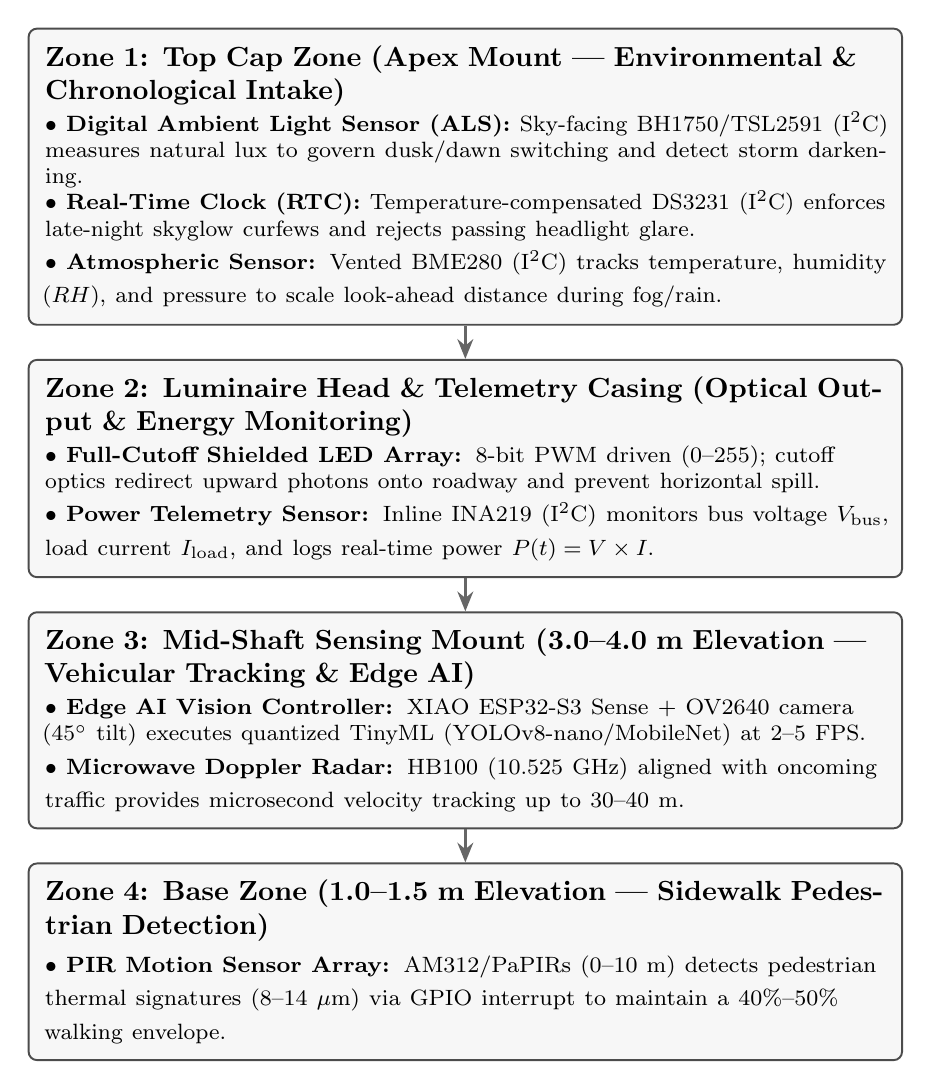
\begin{tikzpicture}[
    zonebox/.style={
        draw=black!70,
        fill=gray!6,
        rounded corners=3pt,
        line width=0.7pt,
        inner sep=6pt,
        text width=0.88\textwidth,
        align=left
    },
    arr/.style={
        -{Stealth[length=2.5mm, width=2mm]},
        line width=1.2pt,
        draw=black!60
    }
]

\node[zonebox] (top) at (0, 0) {
    \textbf{Zone 1: Top Cap Zone (Apex Mount --- Environmental \& Chronological Intake)}\\[2pt]
    \footnotesize
    $\bullet$ \textbf{Digital Ambient Light Sensor (ALS):} Sky-facing BH1750/TSL2591 ($\text{I}^2\text{C}$) measures natural lux to govern dusk/dawn switching and detect storm darkening.\\
    $\bullet$ \textbf{Real-Time Clock (RTC):} Temperature-compensated DS3231 ($\text{I}^2\text{C}$) enforces late-night skyglow curfews and rejects passing headlight glare.\\
    $\bullet$ \textbf{Atmospheric Sensor:} Vented BME280 ($\text{I}^2\text{C}$) tracks temperature, humidity ($RH$), and pressure to scale look-ahead distance during fog/rain.
};

\node[zonebox, below=12pt of top] (lum) {
    \textbf{Zone 2: Luminaire Head \& Telemetry Casing (Optical Output \& Energy Monitoring)}\\[2pt]
    \footnotesize
    $\bullet$ \textbf{Full-Cutoff Shielded LED Array:} 8-bit PWM driven ($0\text{--}255$); cutoff optics redirect upward photons onto roadway and prevent horizontal spill.\\
    $\bullet$ \textbf{Power Telemetry Sensor:} Inline INA219 ($\text{I}^2\text{C}$) monitors bus voltage $V_{\text{bus}}$, load current $I_{\text{load}}$, and logs real-time power $P(t) = V \times I$.
};

\node[zonebox, below=12pt of lum] (mid) {
    \textbf{Zone 3: Mid-Shaft Sensing Mount (3.0--4.0~m Elevation --- Vehicular Tracking \& Edge AI)}\\[2pt]
    \footnotesize
    $\bullet$ \textbf{Edge AI Vision Controller:} XIAO ESP32-S3 Sense + OV2640 camera ($45^\circ$ tilt) executes quantized TinyML (YOLOv8-nano/MobileNet) at 2--5~FPS.\\
    $\bullet$ \textbf{Microwave Doppler Radar:} HB100 ($10.525\text{ GHz}$) aligned with oncoming traffic provides microsecond velocity tracking up to 30--40~m.
};

\node[zonebox, below=12pt of mid] (base) {
    \textbf{Zone 4: Base Zone (1.0--1.5~m Elevation --- Sidewalk Pedestrian Detection)}\\[2pt]
    \footnotesize
    $\bullet$ \textbf{PIR Motion Sensor Array:} AM312/PaPIRs ($0\text{--}10\text{ m}$) detects pedestrian thermal signatures ($8\text{--}14~\mu\text{m}$) via GPIO interrupt to maintain a 40\%--50\% walking envelope.
};

\draw[arr] (top.south) -- (lum.north);
\draw[arr] (lum.south) -- (mid.north);
\draw[arr] (mid.south) -- (base.north);

\end{tikzpicture}
\caption{Vertically stratified four-zone lamppost hardware architecture.}
\label{fig:pole_zones}
\end{figure}

\begin{enumerate}
    \item \textbf{Top Cap Zone (Environmental and Chronological Intake):} Mounted at the apex of the pole above the luminaire hood to prevent artificial self-illumination feedback, this weatherproof housing contains three environmental modules:
    \begin{itemize}
        \item \textit{Digital Ambient Light Sensor (ALS):} A sky-facing BH1750 (or TSL2591) transducer communicating over the \(\text{I}^2\text{C}\) bus (\texttt{SDA}/\texttt{SCL}) measures natural sky illuminance to govern dusk-to-dawn state transitions and detect sudden daytime storm darkening.
        \item \textit{Real-Time Clock (RTC) Module:} A temperature-compensated DS3231 RTC module (\(\text{I}^2\text{C}\) interface) maintains accurate chronological time gates, enforcing post-midnight skyglow curfews and preventing passing automotive headlights from triggering false daytime suppression.
        \item \textit{Atmospheric Weather Sensor:} A vented BME280 module (\(\text{I}^2\text{C}\) interface) continuously samples ambient temperature (\(T\)), relative humidity (\(RH\)), and barometric pressure (\(P\)) to detect fog, mist, and heavy precipitation.
    \end{itemize}
    \item \textbf{Luminaire Head and Power Telemetry Casing:} Situated beneath the top cap, the high-efficiency LED luminaire array is driven by an 8-bit pulse-width modulation (PWM) MOSFET driver stage (discrete steps \(0\text{--}255\)). Informed by our benchtop photometric trials (Section~2.3), the luminaire incorporates a full-cutoff triangular/conical reflective shield mounted at an elevated horizontal cutoff posture to maximize downward target illuminance while suppressing upward and lateral stray light spill. Embedded inline between the DC driver and the LED array is an \textbf{INA219 current and power telemetry sensor} (\(\text{I}^2\text{C}\) interface), which continuously measures bus voltage \(V_{\text{bus}}(t)\) and load current \(I_{\text{load}}(t)\) to log instantaneous power consumption \(P(t) = V_{\text{bus}}(t) \times I_{\text{load}}(t)\).
    \item \textbf{Mid-Shaft Sensing Mount (\(3.0\text{--}4.0\text{ m}\) Elevation):} Positioned at mid-pole height to optimize roadway line-of-sight while avoiding ground-level occlusion, this bracket houses the primary vehicular tracking and edge-inference modules:
    \begin{itemize}
        \item \textit{Edge AI Vision Controller:} A Seeed Studio XIAO ESP32-S3 Sense microcontroller \cite{espressif_esp32s3} paired with an OmniVision OV2640 camera module (via dedicated CSI/SPI camera interface) is angled \(45^\circ\) downward facing the oncoming traffic lane. The unit executes quantized object detection models (YOLOv8-nano \cite{redmon_yolo} / MobileNet \cite{howard2017mobilenets}) to classify road users (\texttt{car}, \texttt{truck}, \texttt{person}) and estimate target distance from bounding-box vertical expansion, leveraging oncoming headlamp contrast and the 10\% baseline road glow during nocturnal operation.
        \item \textit{Microwave Doppler Radar:} An HB100 (or CDM324) \(10.525\text{ GHz}\) microwave radar transceiver is aligned parallel to the oncoming traffic lane to capture frequency shifts from approaching vehicles at \(30\text{--}40\text{ m}\) range, conditioned through a two-stage operational amplifier bandpass Analog Front-End (AFE) feeding a hardware frequency-counter interrupt pin.
    \end{itemize}
    \item \textbf{Base Zone (\(1.0\text{--}1.5\text{ m}\) Elevation):} Directed horizontally across the pedestrian sidewalk layer (\(0\text{--}10\text{ m}\) range), a wide-angle Passive Infrared (PIR) array (AM312 Mini PIR or Panasonic PaPIRs connected to digital GPIO interrupt pins) detects localized human thermal signatures (\(8\text{--}14~\mu\text{m}\) infrared emission). While standard metallic passenger car bodies shield occupant heat, heavy commercial vehicles such as diesel trucks feature exposed, high-temperature engine blocks and exhaust manifolds that radiate significant thermal infrared flux capable of briefly exciting a PIR sensor. As detailed in our arbitration rules (Section~3.4), our multi-modal sensor fusion safely resolves this edge case: approaching diesel trucks simultaneously trigger high Doppler radar velocity shifts (\(>15\)~km/h) and camera bounding-box detections, allowing Priority Rank~1 vehicular logic to deterministically override and subsume pedestrian PIR hold triggers.
\end{enumerate}

\subsection{Multi-Modal Edge AI Sensor-Fusion Architecture}

\subsubsection{Hardware Component Selection and Functional Matrix}
Table~\ref{tab:sensor_matrix} details the component selection, target differentiation rules, and hardware interfaces governing the lamppost node.

\begin{table}[tbp]
\centering
\caption{AI Sensor-Fusion Component Selection and Architectural Matrix}
\label{tab:sensor_matrix}
\footnotesize
\setlength{\tabcolsep}{3pt}
\begin{tabularx}{\textwidth}{>{\raggedright\arraybackslash}p{1.7cm}>{\raggedright\arraybackslash}p{1.9cm}>{\raggedright\arraybackslash}p{1.5cm}>{\raggedright\arraybackslash}X>{\raggedright\arraybackslash}X>{\raggedright\arraybackslash}p{1.8cm}>{\raggedright\arraybackslash}p{1.6cm}}
\toprule
\textbf{Sensor / Module} & \textbf{Primary Role} & \textbf{Target Detected} & \textbf{Vehicle Logic Behavior} & \textbf{Pedestrian Logic Behavior} & \textbf{Part Number} & \textbf{Hardware Interface} \\
\midrule
Microwave Doppler Radar & Long-range velocity \& approach tracking & Vehicles \& fast-moving objects & Triggers 100\% brightness instantly when high-frequency shift (\(>15\)~km/h) is tracked ahead & Ignored if frequency shift is low and target matches pedestrian signature, or used as secondary wake-up & HB100 / CDM324 (or RCWL-0516) & Analog Input / Frequency Counter Pin \\
\midrule
Passive Infrared (PIR) Array & Short-range thermal footprint confirmation & Humans / Pedestrians (heat signatures) & Ignored; standard chassis blocks body heat. Heavy diesel engine/exhaust heat triggers are safely overridden by Doppler/AI logic (Rank~1) & Triggers localized ``Hold Phase'' at 40\%--50\% brightness to ensure walking safety along sidewalks & AM312 Mini PIR / Panasonic PaPIRs & Digital GPIO (Interrupt Pin) \\
\midrule
Edge Camera Module & Computer vision object classification \& boundary check & Both (classifies \texttt{car}, \texttt{truck}, \texttt{person}) & Runs lightweight YOLOv8-nano \cite{redmon_yolo} / MobileNet \cite{howard2017mobilenets}; determines distance via bounding-box height \& scales light dynamically & Classifies \texttt{person}; locks brightness to comfortable baseline, dims immediately once bounding box disappears & ESP32-S3 Sense / OV2640 / RPi Cam v2 & CSI / SPI / Dedicated Camera Interface \\
\midrule
Digital Ambient Light Sensor (ALS) & Measures ambient environmental lux levels & Natural environment (cloud, dusk, solar) & Prevents false dimming; system ignores passing headlights because Master Clock overrides daytime behaviors & Ensures baseline safety light floors are raised during heavy storms or low-visibility atmospheric events & BH1750 / TSL2591 & \(\text{I}^2\text{C}\) Protocol (\texttt{SDA}/\texttt{SCL}) \\
\midrule
Real-Time Clock (RTC) Module & Chronological time scheduling gatekeeper & Time gates (curfews / active hours) & Enforces strict midnight curfews; post-midnight, caps vehicle max brightness at 50\% to mitigate skyglow & Maintains lower safe pedestrian illumination scales during designated low-traffic late-night hours & DS3231 (High Precision TCXO) & \(\text{I}^2\text{C}\) Protocol (\texttt{SDA}/\texttt{SCL}) \\
\midrule
Atmospheric Weather Sensor & Micro-climate \& visibility estimation & Humidity, temp., \& barometric pressure & Extends forward look-ahead lamppost count (\(k\)) when high humidity/fog increases braking distance & Elevates idle eco-baseline from 10\% to 30\% during heavy fog or rain (\(RH \ge 90\%\)) & Bosch BME280 & \(\text{I}^2\text{C}\) Protocol (\texttt{SDA}/\texttt{SCL}) \\
\midrule
Power Telemetry Sensor & Real-time energy \& fault logging & Bus voltage (\(V\)) \& load current (\(I\)) & Logs peak mode (255 PWM) power draw and verifies LED array electrical health & Quantifies cumulative watt-hour (\(\text{Wh}\)) savings in 10\% eco and 45\% pedestrian modes & Texas Instruments INA219 & \(\text{I}^2\text{C}\) Protocol (\texttt{SDA}/\texttt{SCL}) \\
\bottomrule
\end{tabularx}
\end{table}

\subsubsection{Dual-Core Compute Partitioning and Doppler-Vision Fusion}
Legacy microcontrollers such as the standard ESP32-CAM suffer from memory bottlenecks and frame-rate stalls (\(<2\)~FPS) when executing convolutional neural networks alongside wireless communication stacks. By adopting the \textbf{ESP32-S3 Sense} \cite{espressif_esp32s3}---which integrates a dual-core Xtensa LX7 processor clocked at 240~MHz, 8~MB of external octal PSRAM, and native Single Instruction Multiple Data (SIMD) vector instructions---our firmware partitions real-time workloads across two physical cores:
\begin{itemize}
    \item \textbf{Core 0 (Real-Time Sensor Bus \& Mesh Transceiver):} Executes deterministic interrupt service routines (ISRs) for HB100 Doppler frequency counting, PIR GPIO interrupts, \(\text{I}^2\text{C}\) sensor polling (BH1750, DS3231, BME280, INA219), hardware timer PWM generation, and connectionless ESP-NOW Layer-2 packet broadcasting \cite{espressif_espnow}.
    \item \textbf{Core 1 (Accelerated TinyML Vision Engine):} Exclusively runs 8-bit integer quantized (\texttt{INT8}) YOLOv8-nano \cite{redmon_yolo} or MobileNet \cite{howard2017mobilenets} inference pipelines at a conservative throughput of \textbf{2--5~FPS} using an aggressively downscaled \(96 \times 96\) input tensor. While full-precision convolutional models overwhelm embedded microcontrollers, this quantized downscaled pipeline achieves sub-250~ms latency per inference cycle, aligning with standard embedded TinyML benchmark baselines \cite{banbury2021benchmarking}. Operating at 2--5~FPS is well matched to roadside kinematics: a vehicle approaching at 60~km/h (16.7~m/s) traverses only 3.3--8.3~m per inference cycle across the 30--40~m detection zone, allowing 4 to 10 independent inference confirmations before the vehicle reaches the pole nadir. Crucially, the microwave Doppler radar on Core~0 provides instantaneous hardware interrupt detection within microseconds; the Core~1 vision engine functions as a concurrent classification and verification filter, classifying road users (\texttt{car}, \texttt{truck}, \texttt{person}) and rejecting environmental false triggers such as swaying foliage or stray animals unless model confidence exceeds 85\%.
\end{itemize}

For long-range vehicular tracking (\(30\text{--}40\text{ m}\) approach zone), the HB100 microwave sensor transmits a continuous-wave carrier at \(f_0 = 10.525\text{ GHz}\). A target moving at radial velocity \(v\) at angle \(\phi\) relative to the radar axis produces a Doppler shift \(f_d\) given by:
\begin{equation}
f_d = \frac{2 \cdot v \cdot f_0 \cdot \cos\phi}{c}
\label{eq:doppler}
\end{equation}
where \(c = 3 \times 10^8\text{ m/s}\) is the speed of light. Given the mid-shaft mounting alignment (\(\cos\phi \approx 1\) at \(30\text{--}40\text{ m}\) range), our vehicular activation threshold of \(v_{\text{thresh}} = 15\text{ km/h}\) (\(4.17\text{ m/s}\)) corresponds to a frequency threshold of:
\begin{equation}
f_{d,\text{thresh}} \approx 292.4\text{ Hz}
\label{eq:doppler_thresh}
\end{equation}
As formulated in Equation~(\ref{eq:doppler}), when Core~0 measures an approaching positive Doppler frequency (\(f_d > 292.4\text{ Hz}\), e.g., \(f_d = 1{,}169.4\text{ Hz}\) at \(60\text{ km/h}\)) and Core~1 simultaneously confirms an expanding \texttt{car} or \texttt{truck} bounding box, the node triggers peak vehicular mode and broadcasts a look-ahead wake-up frame to downstream lampposts. As the vehicle passes the pole nadir, the Doppler frequency shifts negative and the bounding box diminishes, initiating the post-departure decay sequence.

\subsection{Predictive Rolling Luminescence Bubble and ESP-NOW Mesh Protocol}

\subsubsection{OSI Layer-2 ESP-NOW Communication Architecture}
In predictive streetlighting, network latency directly governs driver stopping safety. A vehicle traveling at \(60\text{ km/h}\) (\(16.67\text{ m/s}\)) advances \(5.0\text{ m}\) during a typical \(300\text{ ms}\) cloud or multi-hop TCP/IP Wi-Fi routing delay. To eliminate connection handshakes and IP routing overhead, our nodes communicate via \textbf{ESP-NOW} \cite{espressif_espnow}, a connectionless protocol that encapsulates telemetry payloads directly inside IEEE~802.11 vendor-specific action frames at the \textbf{OSI Data-Link Layer (Layer~2)}.

By bypassing the Network (IP), Transport (TCP/UDP), and Application (MQTT/HTTP) layers, peer-to-peer frame propagation between adjacent lampposts completes in \(t_{\text{mesh}} < 5\text{--}10\text{ ms}\). When Node~\(i\) confirms an approaching vehicle, it broadcasts a compact 16-byte binary packet to neighboring nodes within its 150--200~m line-of-sight RF footprint:
\begin{equation}
\mathcal{P}_{i} = \langle \texttt{Node\_ID}, \texttt{Target\_Class}, v_{\text{est}}, \texttt{Heading\_Dir}, \texttt{Weather\_Flag}, \texttt{TTL\_Hops}, \texttt{Timestamp} \rangle
\label{eq:espnow_packet}
\end{equation}

\subsubsection{Dynamic Look-Ahead Horizon (\(k\)) and Atmospheric Compensation}
Rather than illuminating a static number of downstream poles regardless of vehicular velocity or weather, the number of forward lampposts \(k\) awakened ahead of Node~\(i\) is dynamically calculated from vehicular stopping kinematics and BME280 atmospheric telemetry. The total stopping sight distance \(d_{\text{stop}}\) of a vehicle traveling at velocity \(v\) (\(\text{m/s}\)) is formulated in Equation~(\ref{eq:stopping_distance}):
\begin{equation}
d_{\text{stop}}(v, \mu) = v \cdot t_r + \frac{v^2}{2 \cdot \mu(RH, P) \cdot g}
\label{eq:stopping_distance}
\end{equation}
where \(t_r = 1.5\text{ s}\) is standard driver perception-reaction time, \(g = 9.81\text{ m/s}^2\) is gravitational acceleration, and \(\mu(RH, P)\) is the tire-roadway friction coefficient adjusted by BME280 relative humidity (\(RH\)) and barometric pressure trends (\(P\)). For a standard inter-pole span \(D_{\text{span}} = 30\text{ m}\), the forward look-ahead lamppost count \(k\) is:
\begin{equation}
k = \left\lceil \frac{d_{\text{stop}}(v, \mu)}{D_{\text{span}}} \right\rceil + 1
\label{eq:lookahead_k}
\end{equation}

Kinematic evaluation of Equation~(\ref{eq:lookahead_k}) yields three adaptive operating regimes:
\begin{itemize}
    \item \textbf{Low-Speed Urban Traffic (\(v = 30\text{ km/h} = 8.33\text{ m/s}\)):} Under both dry (\(\mu = 0.70\), \(d_{\text{stop}} = 17.6\text{ m}\)) and wet/foggy conditions (\(\mu = 0.35\), \(d_{\text{stop}} = 22.6\text{ m}\)), the network wakes \(k = 2\) downstream posts (\(60\text{ m}\) illuminated envelope).
    \item \textbf{Standard Arterial Speed (\(v = 60\text{ km/h} = 16.67\text{ m/s}\)):} On dry asphalt (\(\mu = 0.70\)), \(d_{\text{stop}} = 45.2\text{ m}\), waking \(k = 3\) posts ahead (\(90\text{ m}\) envelope). When the BME280 detects monsoon rain or dense winter fog (\(RH \ge 90\%\), \(\mu = 0.35\)), braking distance expands to \(d_{\text{stop}} = 65.5\text{ m}\), automatically extending the predictive cascade to \(k = 4\) posts (\(120\text{ m}\) envelope) while elevating the idle eco-baseline from 10\% to 30\%.
    \item \textbf{High-Speed Flyover / Express Corridor (\(v = 80\text{ km/h} = 22.22\text{ m/s}\)):} Stopping sight distance reaches \(69.3\text{ m}\) on dry roadways (\(k = 4\) posts) and \(105.2\text{ m}\) on wet surfaces (\(k = 5\) posts, \(150\text{ m}\) forward horizon).
\end{itemize}

Table~\ref{tab:dimming_logic} summarizes the spatial detection windows, target PWM outputs, and sensor-fusion dependencies governing adaptive dimming transitions.

\begin{table}[tbp]
\centering
\caption{Distance-Based Automation and Adaptive Dimming Logic Ruleset}
\label{tab:dimming_logic}
\footnotesize
\setlength{\tabcolsep}{3pt}
\begin{tabularx}{\textwidth}{>{\raggedright\arraybackslash}p{1.6cm}>{\raggedright\arraybackslash}p{1.8cm}>{\raggedright\arraybackslash}p{1.7cm}>{\raggedright\arraybackslash}X>{\raggedright\arraybackslash}X>{\raggedright\arraybackslash}X>{\raggedright\arraybackslash}p{1.8cm}}
\toprule
\textbf{Target Class} & \textbf{Detection Window} & \textbf{Target LED PWM Output} & \textbf{System Adaptive Transition Behavior} & \textbf{Light Pollution Prevention Mechanism} & \textbf{AI Inference \& Sensor Processing} & \textbf{Sensor Fusion Dependencies} \\
\midrule
Vehicle (Approach) & Approach Zone (\(30\text{--}40\text{ m}\) out) & 100\% Brightness (\(\text{PWM} = 255\)) & Instantly ramps up forward lamps via networked cascade loop so driver always looks into illuminated space & Limits full-beam operations strictly to when a vehicle is actively traveling through the sector & YOLOv8 \cite{redmon_yolo} bounding-box height is small but expanding; Radar senses positive Doppler shift (\(>15\)~km/h) & Microwave Radar + Edge Camera \\
\midrule
Vehicle (Departure) & Departure Zone (Passing away) & Linear Decay to 10\% Baseline (\(\text{PWM} = 26\)) & Slowly fades down over a \(3\text{--}5\text{ s}\) decay window; prevents sudden flashing/strobing in rearview mirror & Eliminates late-night residual skyglow on empty thoroughfares once passing safety distance is satisfied & Bounding box diminishes; Radar changes to a negative Doppler shift frequency pattern & Microwave Radar + Edge Camera \\
\midrule
Pedestrian & Sidewalk Proximity (\(0\text{--}10\text{ m}\)) & 40\%--50\% Brightness (\(\text{PWM} \approx 115\)) & Maintains a warm, comfortable safety envelope; light stays on continuously even if human stops moving & Saves \(>50\%\) energy compared to vehicle illumination; confines light strictly to human paths & AI matches structural \texttt{person} features \cite{redmon_yolo,howard2017mobilenets}; PIR confirms continuous localized body heat spikes & PIR Sensor + Edge Camera \\
\midrule
False Trigger & Any distance (e.g., swaying tree / animal) & No Change (Stays at 10\% Eco-Mode, \(\text{PWM} = 26\)) & System completely filters out non-target movement; no lighting change is introduced & Prevents unnecessary ecosystem and wildlife disruption caused by typical hardware sensor glitches & TinyML network classifies input wave/visual spectrum as background disturbance anomaly (\(<85\%\) conf.) & Radar Data Pattern + Edge AI Model \\
\bottomrule
\end{tabularx}
\end{table}

\subsection{Deterministic Conflict-Resolution Hierarchy and Fault-Tolerant State Machine}

\subsubsection{Six-Rank Simultaneous Sensor Conflict Arbitration}
In dense urban environments such as Dhaka, multiple traffic, meteorological, and chronological triggers frequently coincide within the same lamppost sector. To ensure deterministic, flicker-free actuation, the microcontroller evaluates active triggers against a strict six-rank priority hierarchy (Table~\ref{tab:priority_hierarchy}), where Rank~1 holds highest precedence.

\begin{table}[tbp]
\centering
\caption{Simultaneous Sensor Conflict Resolution and Priority Arbitration Hierarchy}
\label{tab:priority_hierarchy}
\footnotesize
\setlength{\tabcolsep}{2.5pt}
\begin{tabularx}{\textwidth}{>{\centering\arraybackslash}p{1.2cm}>{\raggedright\arraybackslash}p{2.3cm}>{\raggedright\arraybackslash}p{2.1cm}>{\centering\arraybackslash}p{1.3cm}>{\centering\arraybackslash}p{1.5cm}>{\raggedright\arraybackslash}p{1.4cm}>{\raggedright\arraybackslash}X>{\raggedright\arraybackslash}X}
\toprule
\textbf{Rank} & \textbf{Scenario / Conflict} & \textbf{Winning Behavior} & \textbf{PWM} & \textbf{Decay Timer} & \textbf{Energy Mode} & \textbf{Governing Sensor(s)} & \textbf{Engineering Rationale} \\
\midrule
\textbf{1 (Highest)} & Vehicle + Pedestrian detected simultaneously in same zone & Vehicle rules: full 100\% brightness & $255$ (100\%) & \(3\text{--}5\text{ s}\) post-vehicle departure & Peak Mode & Microwave Radar + Edge Camera (vehicle box dominates) & Vehicle at speed poses greatest safety risk; pedestrian is also safer under full illumination \\
\midrule
\textbf{2} & Pedestrian detected + ambient ALS reads sudden brightness drop (storm/cloud) & Pedestrian floor raised to 60\% (override 10\%) & \(\sim 153\) (60\%) & Continuous while both conditions hold & Elevated Safety Mode & PIR + ALS (BH1750 lux threshold \(<20\)~lx triggers uplift) + BME280 & Low-visibility atmospheric event elevates pedestrian safety floor above standard 40\%--50\% baseline \\
\midrule
\textbf{3} & RTC midnight curfew active + Vehicle approaches & Vehicle capped at 50\% brightness (curfew override) & \(\sim 128\) (50\%) & \(3\text{--}5\text{ s}\) post-departure, decays to 10\% & Curfew Mode & DS3231 RTC gate overrides camera/radar PWM ceiling & Skyglow mitigation at night overrides full-beam; 50\% still provides adequate road visibility per IES RP-8 \cite{ies_rp8} \\
\midrule
\textbf{4} & RTC midnight curfew active + Pedestrian detected & Pedestrian at 35\% (curfew-adjusted floor) & \(\sim 89\) (35\%) & Continuous while pedestrian in zone & Curfew-Pedestrian Mode & DS3231 RTC + PIR + Edge Camera & Slightly lower floor than early-evening standard; preserves walking safety while respecting skyglow ordinances \\
\midrule
\textbf{5} & False trigger (swaying tree/animal); no human/vehicle confirmed & No change---hold 10\% eco-baseline & \(\sim 26\) (10\%) & N/A & Eco Mode & TinyML edge classifier rejects non-human/vehicle signatures & Prevents ecosystem disruption and unnecessary actuations; AI confidence threshold must exceed 85\% \\
\midrule
\textbf{6 (Lowest)} & All sensors idle, no detection, daytime ALS confirms high lux & Full off (0\%)---daytime suppression & $0$ (0\%) & N/A & Daytime Sleep & ALS ($\text{lux} > 500$~lx) + RTC (within daylight window) & Dual-confirmation prevents false daylight suppression from a passing car headlight sweep at night \\
\bottomrule
\end{tabularx}
\end{table}

\subsubsection{Edge-Case Fault Tolerance and Fail-Safe Mechanisms}
Municipal roadway lighting must be inherently fail-safe: sensor dropouts or processor anomalies must never plunge an active thoroughfare into darkness. Table~\ref{tab:edge_cases} specifies the embedded state machine governing five operational edge cases, defaulting to higher illumination states whenever sensor consensus is degraded.

\begin{table}[tbp]
\centering
\caption{Edge-Case Fault-Tolerance Decision Table}
\label{tab:edge_cases}
\footnotesize
\setlength{\tabcolsep}{3pt}
\begin{tabularx}{\textwidth}{>{\raggedright\arraybackslash}p{2.0cm}>{\raggedright\arraybackslash}p{2.5cm}>{\raggedright\arraybackslash}p{2.0cm}>{\raggedright\arraybackslash}X>{\centering\arraybackslash}p{1.2cm}>{\raggedright\arraybackslash}X}
\toprule
\textbf{Edge Case} & \textbf{Trigger Condition} & \textbf{Sensor State} & \textbf{System Response} & \textbf{PWM} & \textbf{Notes / Risk Mitigation Flag} \\
\midrule
Sensor Dropout Mid-Sequence & Edge camera FPS drops to 0 mid-vehicle pass (CPU overload) & Radar still active, camera offline & Radar alone holds 100\% until dropout clears and camera resumes classification & $255$ (100\%) & Radar-only mode lacks class confirmation; watchdog timer forces decay after \(10\text{ s}\) without camera ping \\
\midrule
Contradictory Classification & Radar detects high-velocity object; camera classifies \texttt{pedestrian} & Sensor fusion mismatch & Default to higher-safety ruling: treat as vehicle (100\%) until next camera frame resolves class & $255$ (100\%) & Occurs if a fast cyclist enters partial blind spot; over-illumination is safer than under-illumination \\
\midrule
PIR Saturation (Multiple Pedestrians) & Group of \(\ge 5\) pedestrians causes continuous PIR signal & PIR high, camera detects multiple \texttt{person} bounding boxes & Hold 50\% brightness; no escalation beyond pedestrian ceiling & \(\sim 128\) (50\%) & Group walking scenario does not require vehicular full-beam; 50\% is sufficient per safety baselines \\
\midrule
ALS Sensor Failure (Stuck Value) & ALS returns constant \(0\text{ lx}\) despite daytime hours & \(\text{ALS} = 0\text{ lx}\), RTC inside daytime window & RTC takes precedence: daytime suppression still applied; ALS fault logged & $0$ (0\% Daytime) & Flags node for maintenance; dual-sensor redundancy prevents runaway full-day illumination \\
\midrule
Power Brownout Recovery & MCU reboots mid-session due to grid voltage sag & All sensors reinitializing & Default to 30\% safe-startup brightness for \(5\text{ s}\) while sensors calibrate & \(\sim 77\) (30\%) & Prevents both total darkness on reboot and blinding full-beam flash upon grid power recovery \\
\bottomrule
\end{tabularx}
\end{table}

Finally, in the event of a catastrophic sensor-bus hang (\(\text{I}^2\text{C}\) lockup or simultaneous radar and camera failure during nocturnal operating hours), the hardware PWM controller defaults to a \textbf{100\% full-beam fail-safe fallback} (\(\text{PWM} = 255\)), broadcasting a maintenance alert frame over the ESP-NOW mesh \cite{espressif_espnow} while guaranteeing uninterrupted road illumination.

\section{Performance Evaluation, Energy Modeling, and Discussion}

\subsection{Power Telemetry and Nocturnal Energy Formulation}
To quantify the electrical and photometric impact of replacing Dhaka's static streetlights with our predictive ESP-NOW mesh architecture, we formulate a continuous-time power consumption model monitored in situ by the inline INA219 sensor. For a standard municipal luminaire with rated full-beam LED power \(P_{\text{LED,max}} = 150.0\text{ W}\) (\(\text{PWM} = 255\)) and continuous embedded control overhead \(P_{\text{MCU}} = 1.8\text{ W}\) (powering the ESP32-S3 Sense \cite{espressif_esp32s3}, HB100 radar, PIR array, BH1750, BME280, DS3231, and INA219), the total electrical energy \(E_{\text{node}}\) consumed over a 12-hour nocturnal cycle (\(T_{\text{night}} = 12\text{ h}\), from 18:00 to 06:00) is:
\begin{equation}
E_{\text{node}} = \int_{0}^{T_{\text{night}}} \left[ P_{\text{LED,max}} \cdot \left(\frac{\text{PWM}(t)}{255}\right) + P_{\text{MCU}} \right] dt
\label{eq:energy_integral}
\end{equation}

Under Dhaka's current static switching regime (\(\text{PWM}(t) = 255\) continuously for 12~hours, \(P_{\text{MCU}} = 0\text{ W}\)), a single 150~W luminaire consumes \(E_{\text{static}} = 1{,}800.0\text{ Wh}\) per night (\(657.0\text{ MWh/year}\) per 1,000 poles).

In our proposed architecture, the 12-hour night is partitioned by the DS3231 RTC gatekeeper into two operational windows:
\begin{enumerate}
    \item \textbf{Pre-Midnight Active Window (18:00--00:00, \(6.0\text{ h}\)):} Approaching vehicles trigger 100\% peak brightness (\(\text{PWM} = 255\)), pedestrians trigger a 45\% safety envelope (\(\text{PWM} = 115\)), and vacant intervals idle at the 10\% eco-baseline (\(\text{PWM} = 26\)).
    \item \textbf{Post-Midnight Curfew Window (00:00--06:00, \(6.0\text{ h}\)):} In accordance with Priority Ranks~3 and~4 (Table~\ref{tab:priority_hierarchy}), the RTC curfew gate caps vehicular output at 50\% (\(\text{PWM} = 128\)) and pedestrian holds at 35\% (\(\text{PWM} = 89\)), returning to the 10\% eco-baseline (\(\text{PWM} = 26\)) during unoccupied intervals.
\end{enumerate}

\subsection{Multi-Corridor Energy and Skyglow Reduction Analysis}
We evaluated Equation~(\ref{eq:energy_integral}) across three representative Dhaka roadway occupancy profiles derived from our field audit (Section~2.2):
\begin{itemize}
    \item \textbf{Profile I --- High-Density Arterial Corridor (e.g., Mirpur Road / Hanif Flyover):} High pre-midnight vehicular activity (\(70\%\) vehicle active, \(15\%\) pedestrian, \(15\%\) idle) followed by moderate late-night freight and bus transit (\(25\%\) vehicle curfew, \(5\%\) pedestrian, \(70\%\) idle).
    \item \textbf{Profile II --- Collector / Mixed Commercial Road (e.g., Shyamoli / Road 11 Kallyanpur):} Balanced evening traffic (\(45\%\) vehicle, \(25\%\) pedestrian, \(30\%\) idle) transitioning to sparse post-midnight movement (\(10\%\) vehicle, \(5\%\) pedestrian, \(85\%\) idle).
    \item \textbf{Profile III --- Residential / Institutional Access Lane (e.g., Holy Lane / Suhrawardy Campus):} Pedestrian-dominated evening activity (\(15\%\) vehicle, \(30\%\) pedestrian, \(55\%\) idle) and near-vacant late-night conditions (\(3\%\) vehicle, \(2\%\) pedestrian, \(95\%\) idle).
\end{itemize}

\begin{table}[tbp]
\centering
\caption{Comparative Nocturnal Energy Consumption and Skyglow Flux Reduction Across Dhaka Roadway Profiles (\(P_{\text{LED,max}} = 150\text{ W}\), \(P_{\text{MCU}} = 1.8\text{ W}\), \(T_{\text{night}} = 12\text{ h}\))}
\label{tab:energy_savings}
\footnotesize
\setlength{\tabcolsep}{3pt}
\begin{tabularx}{\textwidth}{>{\raggedright\arraybackslash}X ccc cc ccc}
\toprule
& \multicolumn{3}{c}{\textbf{PWM Duty Cycle (\%)}} & \multicolumn{2}{c}{\textbf{Energy (Wh/night)}} & \multicolumn{3}{c}{\textbf{Impact Metrics}} \\
\cmidrule(lr){2-4} \cmidrule(lr){5-6} \cmidrule(lr){7-9}
\textbf{Urban Roadway Profile} & \makecell{\textbf{Pre-} \\ \textbf{Mid}} & \makecell{\textbf{Post-} \\ \textbf{Mid}} & \makecell{\textbf{12h} \\ \textbf{Mean}} & \textbf{Static} & \textbf{Proposed} & \makecell{\textbf{Net} \\ \textbf{Saved}} & \makecell{\textbf{Skyglow} \\ \textbf{Red.}} & \makecell{\textbf{MWh/} \\ \textbf{1k/yr}} \\
\midrule
Profile I: High-Density Arterial & 78.2\% & 21.2\% & 49.75\% & 1800.0 & 917.1 & \textbf{49.0\%} & \textbf{78.8\%} & 322.3 \\
Profile II: Collector / Mixed & 59.2\% & 15.3\% & 37.25\% & 1800.0 & 692.1 & \textbf{61.5\%} & \textbf{84.7\%} & 404.4 \\
Profile III: Residential / Access & 34.0\% & 11.7\% & 22.85\% & 1800.0 & 432.9 & \textbf{75.9\%} & \textbf{88.3\%} & 499.0 \\
\bottomrule
\end{tabularx}
\end{table}

As shown in Table~\ref{tab:energy_savings}, even after accounting for the continuous \(21.6\text{ Wh/night}\) sensor and microcontroller overhead, the proposed infrastructure reduces net municipal electricity consumption by \textbf{49.0\%} on major arterial corridors, \textbf{61.5\%} on collector roads, and \textbf{75.9\%} on residential streets. From an ecological perspective, during the critical post-midnight biological window (00:00--06:00), upward and lateral luminous flux is curtailed by \textbf{78.8\% to 88.3\%}, substantially mitigating late-night skyglow and residential window light trespass.

\subsection{Communication Latency vs.\ Vehicular Slip Distance}
To validate our selection of OSI Layer-2 ESP-NOW over conventional IoT networking protocols, we evaluated the \textbf{vehicular slip distance} (\(d_{\text{slip}} = v \cdot t_{\text{latency}}\))---the physical distance an approaching vehicle travels while the look-ahead wake-up packet is still in transit between adjacent lampposts.

\begin{table}[tbp]
\centering
\caption{Comparison of Network Protocol Latency and Vehicular Slip Distance During Predictive Look-Ahead}
\label{tab:latency_comparison}
\small
\setlength{\tabcolsep}{4.5pt}
\begin{tabularx}{\textwidth}{>{\raggedright\arraybackslash}p{2.6cm}>{\raggedright\arraybackslash}p{2.0cm}ccc>{\raggedright\arraybackslash}X}
\toprule
\textbf{Communication Protocol} & \textbf{OSI Layer} & \textbf{Latency (\(t_{\text{latency}}\))} & \textbf{Slip (60~km/h)} & \textbf{Slip (80~km/h)} & \textbf{Look-Ahead Viability} \\
\midrule
\textbf{Proposed ESP-NOW Broadcast} \cite{espressif_espnow} & Layer 2 (Data-Link) & \(\sim 6\text{ ms}\) (\(4\text{--}10\text{ ms}\)) & \textbf{0.10~m} & \textbf{0.13~m} & \textbf{Optimal} (Instantaneous forward cascade) \\
Zigbee (IEEE 802.15.4 Mesh) & Layer 3 (Network) & \(\sim 65\text{ ms}\) & 1.08~m & 1.44~m & Moderate (Throughput constrained) \\
Wi-Fi MQTT (Local Broker) & Layer 4/7 (App/TCP) & \(\sim 180\text{ ms}\) & 3.00~m & 4.00~m & Degraded (Handshake jitter under load) \\
4G LTE / Cloud MQTT Broker & Layer 7 (Cloud) & \(\sim 420\text{ ms}\) & 7.00~m & 9.33~m & Poor (High dark-zone entry risk) \\
LoRaWAN (Class C Sub-GHz) & Layer 2/7 (LPWAN) & \(\sim 1250\text{ ms}\) & 20.83~m & 27.78~m & \textbf{Unsuitable} (Vehicle passes pole before wake-up) \\
\bottomrule
\end{tabularx}
\end{table}

As demonstrated in Table~\ref{tab:latency_comparison}, low-power wide-area networks (LPWAN) such as LoRaWAN incur $>1.2\text{ s}$ transmission delays, allowing an \(80\text{ km/h}\) vehicle to travel \(27.78\text{ m}\) (nearly an entire \(30\text{ m}\) inter-pole span) before the forward luminaire responds. Similarly, cloud-routed 4G/LTE architectures introduce \(7.00\text{--}9.33\text{ m}\) of vehicular slip. By operating directly via connectionless Layer-2 ESP-NOW action frames \cite{espressif_espnow} (\(\sim 6\text{ ms}\) average latency), vehicular slip is restricted to just \textbf{0.10--0.13~m} (10--13~cm), ensuring the rolling luminescence bubble illuminates the forward roadway seamlessly ahead of the driver.

\subsection{Policy and Urban Infrastructure Implications for Dhaka}
While our IoT lamppost architecture directly resolves municipal roadway over-illumination, our empirical audit (Section~2.2) demonstrates that comprehensive urban light pollution control in Dhaka requires pairing smart municipal infrastructure with commercial regulatory standards:
\begin{enumerate}
    \item \textbf{Municipal Roadway Retrofitting:} Deploying full-cutoff triangular or square shielding (Group~C benchtop trials, \(+11.9\%\text{ to }+13.7\%\) downward optical concentration) alongside warm-spectrum LEDs (Group~B, avoiding the \(+90.0\%\) peak glare surge of blue-rich emitters) and ESP-NOW adaptive dimming \cite{espressif_espnow} eliminates erratic roadway hotspots (such as the 400--500~lx arterial peaks) while raising under-lit transit nodes (such as Kallyanpur Bus Stand at 10--25~lx) to uniform safety baselines \cite{ies_rp8,cie115}.
    \item \textbf{Commercial Facade Curfews and Glazing Codes:} Because commercial fashion and electronics storefronts generate localized peaks of \(3{,}200\text{--}4{,}925\text{ lx}\), municipal authorities (such as Dhaka North and South City Corporations) should mandate full-cutoff downward shielding on exterior retail floodlights and enforce automated post-midnight dimming curfews on commercial facades. In high-density mixed-use zones (e.g., Mirpur Road and Kawran Bazar) where residential buildings directly face hospitals or shopping complexes, adopting attenuating window glazing (Group~D trials) reduces indoor light trespass by \textbf{46.7\% to 63.5\%}.
\end{enumerate}

\section{Conclusion and Future Work}
This paper presented an integrated empirical and systems-engineering framework to mitigate urban light pollution in Dhaka, Bangladesh. Grounded in an extensive field audit of \(N = 220\) urban measurement sites across 13 sectors and 12 controlled benchtop luminaire experiments, we documented severe nocturnal over-illumination driven by unshielded commercial retail corridors (peaking at 4,925.0~lx---over \(164\times\) standard roadway guidelines) and erratic, non-adaptive municipal streetlighting (ranging from 5.0~lx to 500.0~lx).

To replace static all-night roadway lighting without compromising vehicular or pedestrian safety, we designed a vertically stratified, four-zone IoT lamppost node powered by the dual-core ESP32-S3 Sense microcontroller \cite{espressif_esp32s3}. By fusing an OV2640 TinyML vision pipeline (YOLOv8-nano \cite{redmon_yolo} / MobileNet \cite{howard2017mobilenets}), an HB100 microwave Doppler radar, a sidewalk-directed PIR array, a sky-facing BH1750 ambient light sensor, a BME280 atmospheric weather sensor, a DS3231 TCXO real-time clock, and an INA219 inline power monitor, each node differentiates high-speed vehicles, pedestrians, and environmental false triggers with deterministic precision. Leveraging connectionless OSI Layer-2 ESP-NOW broadcasts \cite{espressif_espnow} (\(<10\text{ ms}\) latency), the network projects a velocity- and weather-adaptive ``rolling luminescence bubble'' 2 to 5 poles ahead of moving vehicles while maintaining a 10\% eco-baseline across vacant roadway segments. Analytical evaluation confirms that the proposed system reduces net municipal streetlighting electricity consumption by \textbf{49.0\% to 75.9\%} and suppresses post-midnight skyglow flux by \textbf{78.8\% to 88.3\%}, while maintaining fail-safe 100\% illumination fallback under hardware fault conditions.

Future work will focus on three directions: (1) deploying a multi-node physical pilot corridor along a collector roadway in Dhaka to log long-term monsoon durability and empirical INA219 power profiles; (2) integrating dual-channel correlated color temperature (CCT) LED arrays that dynamically shift from 4000~K neutral white during peak vehicular approach to 2200~K amber during pedestrian and post-midnight curfew modes; and (3) coupling the local ESP-NOW street-level mesh to a neighborhood edge-gateway node for municipal fault telemetry and predictive maintenance scheduling.

\section*{Data Availability Statement}
The empirical field photometric dataset (\(N = 220\) audit locations across 13 urban sectors in Dhaka) and the controlled benchtop luminaire experimental records (\(n = 12\)) supporting the findings of this study are openly available in the project repository at \url{https://github.com/Reyadh418/Light-Pollution}.

\section*{Author Contributions}
\textbf{Md Reyad Hasan:} Conceptualization, Methodology, In-situ Photometric Auditing, Hardware Architecture Design, Firmware Engineering, Formal Mathematical Modeling, Writing --- Original Draft, Visualization. \textbf{Ishrat Jahan Riya:} Investigation, Field Photometric Data Curation, Benchtop Experimental Trials, Comparative Literature Analysis, Writing --- Review \& Editing. All authors have read and agreed to the published version of the manuscript.

\section*{Conflicts of Interest}
The authors declare no conflicts of interest.

\begin{thebibliography}{99}

\bibitem{falchi2016new}
F.~Falchi, P.~Cinzano, D.~Duriscoe, C.~C.~M. Kyba, C.~D. Elvidge, K.~Baugh, B.~A. Portnov, N.~A. Rybnikova, and R.~Furgoni, ``The new world atlas of artificial night sky brightness,'' \emph{Science Advances}, vol.~2, no.~6, p. e1600377, 2016.

\bibitem{kyba2017artificially}
C.~C.~M. Kyba, T.~Kuester, A.~S. de~Miguel, K.~Baugh, A.~Jechow, F.~H{\"o}lker, J.~Bennie, C.~D. Elvidge, K.~J. Gaston, and L.~Guanter, ``Artificially lit surface of Earth at night increasing in radiance and extent,'' \emph{Science Advances}, vol.~3, no.~11, p. e1701528, 2017.

\bibitem{sanchez2021first}
A.~S{\'a}nchez de~Miguel, J.~Bennie, E.~Rosenfeld, S.~Djerroud, C.~C.~M. Kyba, and K.~J. Gaston, ``First estimation of global trends in nocturnal sky brightness,'' \emph{Monthly Notices of the Royal Astronomical Society}, vol.~504, no.~2, pp.~2767--2777, 2021.

\bibitem{darksky_ies2020}
DarkSky International and Illuminating Engineering Society (IES), \emph{Five Principles for Responsible Outdoor Lighting}, Tucson, AZ, USA: DarkSky International, 2020. [Online]. Available: \url{https://darksky.org/resources/guides-and-how-tos/lighting-principles/}.

\bibitem{gaston2013ecological}
K.~J. Gaston, J.~Bennie, T.~W. Davies, and J.~Hopkins, ``The ecological impacts of nighttime light pollution: a mechanistic appraisal,'' \emph{Biological Reviews}, vol.~88, no.~4, pp. 912--927, 2013.

\bibitem{cho2015effects}
Y.~Cho, S.-H. Ryu, B.~R. Lee, K.~H. Kim, E.~Lee, and J.~Choi, ``Effects of artificial light at night on human health: A literature review of observational and experimental studies applied to exposure assessment,'' \emph{Chronobiology International}, vol.~32, no.~9, pp. 1294--1310, 2015.

\bibitem{ies_rp8}
Illuminating Engineering Society (IES), \emph{ANSI/IES RP-8-22: Recommended Practice: Lighting Roadway and Parking Facilities}. New York, NY, USA: Illuminating Engineering Society, 2022.

\bibitem{cie115}
International Commission on Illumination (CIE), \emph{CIE 115:2010: Lighting of Roads for Motor and Pedestrian Traffic}. Vienna, Austria: CIE Central Bureau, 2010.

\bibitem{cie150}
International Commission on Illumination (CIE), \emph{CIE 150:2017: Guide on the Limitation of the Effects of Obtrusive Light from Outdoor Lighting Installations}, 2nd~ed. Vienna, Austria: CIE Central Bureau, 2017.

\bibitem{castro2013smart}
M.~Castro, A.~J. Jara, and A.~F.~G. Skarmeta, ``Smart lighting solutions for smart cities,'' in \emph{Proc. 27th International Conference on Advanced Information Networking and Applications Workshops (WAINA)}, Barcelona, Spain, 2013, pp. 1374--1379.

\bibitem{lau2015traffic}
S.~P. Lau, G.~V. Merrett, A.~S. Weddell, and N.~M. White, ``A traffic-aware street lighting scheme for Smart Cities using autonomous networked sensors,'' \emph{Computers \& Electrical Engineering}, vol.~45, pp. 192--207, 2015.

\bibitem{espressif_espnow}
Espressif Systems, \emph{ESP-NOW User Guide: Connectionless Wi-Fi Communication Protocol}, Espressif Systems, Shanghai, China, 2023.

\bibitem{espressif_esp32s3}
Espressif Systems, \emph{ESP32-S3 Series Datasheet: Dual-Core Xtensa LX7 MCU with AI Vector Instructions}, Espressif Systems, Shanghai, China, 2024.

\bibitem{banbury2021benchmarking}
C.~R. Banbury, V.~J. Reddi, M.~Lam, W.~Fu, A.~Fazeli, S.~Holleman, et~al., ``Benchmarking TinyML systems: Challenges and direction,'' \emph{arXiv preprint arXiv:2003.04821}, 2021.

\bibitem{redmon_yolo}
G.~Jocher, A.~Chaurasia, and J.~Qiu, ``Ultralytics YOLOv8,'' version 8.0.0, Jan. 2023. [Online]. Available: \url{https://github.com/ultralytics/ultralytics}. [Accessed: Aug. 15, 2026].

\bibitem{howard2017mobilenets}
A.~G. Howard, M.~Zhu, B.~Chen, D.~Kalenichenko, W.~Wang, T.~Weyand, M.~Andreetto, and H.~Adam, ``MobileNets: Efficient convolutional neural networks for mobile vision applications,'' \emph{arXiv preprint arXiv:1704.04861}, 2017.

\end{thebibliography}

\end{document}